\documentclass[10pt,letterpaper,landscape]{article}

\usepackage[margin=0.75in]{geometry}
\usepackage{fancyhdr}
\usepackage{multicol}
\usepackage{listings}
\usepackage{color}
\usepackage{graphicx}
\usepackage{amsmath}

\setlength{\parindent}{0pt}

\definecolor{dkgreen}{rgb}{0,0.6,0}
\definecolor{gray}{rgb}{0.5,0.5,0.5}
\definecolor{mauve}{rgb}{0.58,0,0.82}

\lstset{frame=tb,
		language=C++,
		aboveskip=1mm,
		belowskip=1mm,
		showstringspaces=false,
		columns=flexible,
		basicstyle={\small\ttfamily},
		numbers=none,
		numberstyle=\tiny\color{gray},
		keywordstyle=\color{dkgreen},
		commentstyle=\color{mauve},
		breaklines=true,
		breakatwhitespace=true,
		tabsize=2
}

\pagestyle{fancy}
\lhead{University of Illinois at Urbana-Champaign: VIM - Help poor children!}
\rhead{\thepage}
\cfoot{} % suppress page number at bottom

\begin{document}

% cover page

\thispagestyle{empty}

\begin{center}
    
\includegraphics[scale=0.75]{logo.png} \\
    \vspace{20mm}
    {\Huge \textbf{ICPC World Finals 2019}} \\
    \vspace{10mm}
    {\LARGE \textit{Team Reference Document}} \\
    \vspace{30mm}
    {\LARGE University of Illinois at Urbana-Champaign} \\
    \vspace{5mm}
    {\LARGE VIM - Help poor children!} \\
    \vspace{30mm}
    {\Large \textbf{Coaches:} Alan Mattox Beckman Jr, Zhengkai Wu} \\
	\vspace{5mm}
	{\Large \textbf{Contestants:} Lan Dao, Jiacheng Liu, Zexuan Zhong}
\end{center}

\newpage

\begin{multicols}{2}

\tableofcontents

\newpage

\section{Getting Started}
\subsection{Vimrc}
\begin{lstlisting}
syntax on
set nu
set ruler
set autoindent
set smartindent
set expandtab
set tabstop=4
set shiftwidth=4
\end{lstlisting}
\subsection{C++ Grammar, STL}
\begin{lstlisting}
string s; getline(cin, s);  // read one line
stringstream ss(s); int a; ss >> a; ss.ignore();  // read comma-separated integers

bool valid = next_permutation(b, e);
bool found = binary_search(b, e, val, cmp);
auto it = lower_bound(b, e, val, cmp);  // first element >= val
auto it = upper_bound(b, e, val, cmp);  // first element > val
stable_sort(b, e, cmp);  // preserve relative order of eq vals
unique(b, e);

struct Cmp { bool operator() (T &a, T &b) { return true; } };
set<T,Cmp> s;
bool cmp (T &a, T &b) { return true; }
set<T,decltype(cmp)> s(cmp);
auto cmp = [](T &a, T &b) -> bool { return true; }
set<T,decltype(cmp)> s(cmp);

map<int,int> m;
m.find(val) == m.end()
for (auto p : m) { key = p.F; value = p.S; }

priority_queue<T, vector<T>, Cmp> pq;
\end{lstlisting}
\section{Data Structures}
\subsection{Segment Tree 2D}
\begin{lstlisting}
// Supported:
// - Add a value v to cell (x, y)
// - Get the sum in rectangle with top left corner 
// (x1, y1) and bottom right corner (x2, y2)
void build_y(int k_x, int k_y, int l, int r) {
    if (l == r) { 
        t[k_x][k_y] = 0; 
        return;
    }
    int mid = (l + r) >> 1;
    build_y(k_x, k_y * 2, l, mid);
    build_y(k_x, k_y * 2 + 1, mid + 1, r);
    t[k_x][k_y] = 0;
}
void build_x(int k, int l, int r) {
    build_y(k, 1, 1, n);
    if (l == r) return;
    int mid = (l + r) >> 1;
    build_x(k * 2, l, mid);
    build_x(k * 2 + 1, mid + 1, r);
}
void update_y(int k_x, int l_x, int r_x, int k_y, int l_y, int r_y, int y, int v) {
    if (y < l_y || r_y < y) return;
    if (l_y == r_y) {
        if (l_x == r_x)
            t[k_x][k_y] += v;
        else
            t[k_x][k_y] = t[k_x * 2][k_y] + t[k_x * 2 + 1][k_y];
        return;
    }
    int mid = (l_y + r_y) >> 1;
    update_y(k_x, l_x, r_x, k_y * 2, l_y, mid, y, v);
    update_y(k_x, l_x, r_x, k_y * 2 + 1, mid + 1, r_y, y, v);
    t[k_x][k_y] = t[k_x][k_y * 2] + t[k_x][k_y * 2 + 1];
}
void update_x(int k, int l, int r, int x, int y, int v) {
    if (x < l || r < x) return;
    if (l == r) {
        update_y(k, l, r, 1, 1, n, y, v);
        return;
    }
    int mid = (l + r) >> 1;
    update_x(k * 2, l, mid, x, y, v);
    update_x(k * 2 + 1, mid + 1, r, x, y, v);
    update_y(k, l, r, 1, 1, n, y, v);
}
int get_y(int k_x, int k_y, int l, int r, int y1, int y2) {
    if (y2 < l || r < y1) return 0;
    if (y1 <= l && r <= y2) return t[k_x][k_y];
    int mid = (l + r) >> 1;
    return get_y(k_x, k_y * 2, l, mid, y1, y2) +
           get_y(k_x, k_y * 2 + 1, mid + 1, r, y1, y2); 
}
int get_x(int k, int l, int r, int x1, int x2, int y1, int y2) {
    if (r < x1 || x2 < l) return 0;
    if (x1 <= l && r <= x2)
        return get_y(k, 1, 1, n, y1, y2);
    int mid = (l + r) >> 1;
    return get_x(k * 2, l, mid, x1, x2, y1, y2) +
           get_x(k * 2 + 1, mid + 1, r, x1, x2, y1, y2); 
}
\end{lstlisting}
\subsection{Persistent Segment Tree}
\begin{lstlisting}
struct Node {
    Node() = default;
    Node(int l, int r, int v) : left(l), right(r), val(v) {}
    int left, right, val;
};
int build(int k, int l, int r) {
    tree[k].val = 0;
    if (l == r) return k;
    tree[k].left = ++num_node;
    tree[k].right = ++num_node;
    int mid = (l + r) >> 1;
    build(tree[k].left, l, mid);
    build(tree[k].right, mid + 1, r);
    return k;
}
int update(int k, int l, int r, int i, int v) {
    int K = ++num_node;
    if (l == r) {
        tree[K].val = tree[k].val + v;
        return K;
    }
    tree[K].left = tree[k].left;
    tree[K].right = tree[k].right;
    int mid = (l + r) >> 1;
    if (i <= mid)
        tree[K].left = update(tree[K].left, l, mid, i, v);
    else
        tree[K].right = update(tree[K].right, mid + 1, r, i, v);
    tree[K].val = tree[tree[K].left].val + tree[tree[K].right].val;
    return K;
}
\end{lstlisting}
\subsection{Splay Tree + Link Cut Tree}
\begin{lstlisting}
inline void Zig(int x) {
    int y = fa(x), z = fa(y);
    if (y == lc(z)) lc(z) = x;
    else if (y == rc(z)) rc(z) = x;
    fa(x) = z;
    lc(y) = rc(x); fa(rc(x)) = y;
    rc(x) = y; fa(y) = x;
    Updata(y);
}
inline void Zag(int x) {
    int y = fa(x), z = fa(y);
    if (y == lc(z)) lc(z) = x;
    else if (y == rc(z)) rc(z) = x;
    fa(x) = z;
    rc(y) = lc(x); fa(lc(x)) = y;
    lc(x) = y; fa(y) = x;
    Updata(y);
}
#define root(x) (lc(fa(x)) != x && rc(fa(x)) != x)
inline void Splay(int x) // (int &root,int x) {
    int y, z; 
    Relax(x); // reverse and release marks
    while (!root(x)) // fa(x) != fa(root)
    {
        y = fa(x); z = fa(y);
        if (root(y))
            if (x == lc(y)) Zig(x);
            else Zag(x);
        else if (y == lc(z))
            if (x == lc(y)) Zig(y), Zig(x);
            else Zag(x), Zig(x);
        else if (x == rc(y)) Zag(y), Zag(x);
            else Zig(x), Zag(x);
    }
    Updata(x); // root = x;
}
inline int Expose(int x) {
    int y;
    for (y = 0; x; y = x, x = fa(x))
    {
        Splay(x); rc(x) = y;
        Updata(x);
    }
    return y;
}
\end{lstlisting}
\subsection{K-th Number (Huafen Tree)}
\begin{lstlisting}
// d[1][i]: value of the i-th element (unique)
void Build(int l,int r,int h) {
     if (l==r) return;
     int m=l+r>>1,i,lpos=l,rpos=m+1,ss=0;
     for (i=l;i<=r;i++)
     {
         if (d[h][i]<=m)
         {
            ss++;
            d[h+1][lpos++]=d[h][i];
         }
         else d[h+1][rpos++]=d[h][i];
         s[h][i]=ss;
     }
     Build(l,m,h+1);
     Build(m+1,r,h+1);
}
inline int Ask(int l,int r,int h,int x,int y,int k) {
    if (l==r) return a[sa[d[h][l]]];
    int l1,l2,m=l+r>>1;
    l1=(x!=l)?s[h][x-1]:0;
    l2=s[h][y];
    if (k<=l2-l1) return Ask(l,m,h+1,l+l1,l+l2-1,k);
    else return Ask(m+1,r,h+1,m+1+x-l-l1,m+1-l-l2+y,k-l2+l1);
}
\end{lstlisting}
\subsection{Mo's Algorithm}
\begin{lstlisting}
// The array is 1-based
bool cmp_mo(Query i, Query j) {
    int s = (int) sqrt(n);
    return ((i.l - 1) / s < (j.l - 1) / s || ((i.l - 1) / s == (j.l - 1) / s && i.r < j.r));
}
\end{lstlisting}
\section{Graph Theory}
\subsection{Dinic}
\begin{lstlisting}
bool make_level() {
	for (int i = 0; i < n; i ++) {
		nodes[i].level = -1;
	}
	queue<Node*> queue;
	queue.push(&nodes[0]);
	nodes[0].level = 0;
	while (!queue.empty()) {
		Node* node = queue.front();
		queue.pop();
		for (Edge *edge = node->head; edge; edge = edge->next) {
			if (nodes[edge->v].level == -1 && edge->c) {
				nodes[edge->v].level = node->level + 1;
				queue.push(&nodes[edge->v]);
			}
		}
	}
	return nodes[n-1].level != -1;
}
int find(int u, int key) {
	if (u == n-1) return key;
	for (Edge *edge = nodes[u].head; edge; edge = edge->next) {
		if (nodes[edge->v].level == nodes[u].level + 1 && edge->c) {
			int flow = find(edge->v, min(key, edge->c));
			if (flow) {
				edge->c -= flow;
				edge->rev->c += flow;
				return flow;
			}
		}
	}
	return 0;
}
int dinic() {
	int ans = 0;
	int flow;
	while (make_level())
		while ((flow = find(0, INT_MAX)))
			ans += flow;
	return ans;
}
\end{lstlisting}
\subsection{Min Cost Max Flow}
\begin{lstlisting}
bool spfa() {
    int h, t, x, y;
    rep(i, T) dis[i] = inf, at[i] = 0;
    q[t = 1] = S; dis[S] = 0; at[S] = 1;
    h = 0;
    while (h != t) {
        ++h; if (h > 400) h = 1;
        x = q[h];
        foredge(i, x) if (e[i].c > 0) {
            y = e[i].a;
            if (dis[y] > dis[x] + e[i].v) {
                dis[y] = dis[x] + e[i].v;
                pre[y] = i;
                if (!at[y]) {
                    ++t; if (t > 400) t = 1;
                    q[t] = y; at[y] = 1;
                }
            }
        }
        at[x] = 0;
    }
    return dis[T] != inf;
}
int main() {
    int ans = 0;
    while (spfa()) {
        ans += dis[T];
        for (int x = T; x; x = e[pre[x] ^ 1].a) {
            e[pre[x]].c--; e[pre[x] ^ 1].c++;
        }
    }
}
\end{lstlisting}
\subsection{Minimum Vertex Cover Bipartite Graph}
\begin{lstlisting}
void alternate(int u) {
    lmvc[u] = false;
    for (int v : rhs)
        if (c[u][v]) {
            rmvc[v] = true;
            if (rmatch[v] && lmvc[rmatch[v]])
                alternate(rmatch[v]);
        }
}

void MVC() {
    max_matching();
    for (int u : rhs) rmvc[u] = false;
    for (int u : lhs) lmvc[u] = (lmatch[u] != 0);
    for (int u : lhs)
        if (!lmvc[u]) alternate(u);
}
\end{lstlisting}
\subsection{Cut Node / Edge}
\begin{lstlisting}
enum {NOT_VISITED, IN_STACK, VISITED};
set<int> cut_node;
set<Edge*> cut_edge;
vector<int> status(n, 0);
vector<int> dfn(n, 0);
vector<int> low(n, 0);
pair<set<int>,set<Edge*>> cut_node_edge() {
	for (int i = 0; i < n; i ++)
		if (status[i] == NOT_VISITED)
			cut_node_edge(i, -1, 0);
	return {cut_node, cut_edge};
}
void cut_node_edge(int node, int parent, int depth) {
	status[node] = IN_STACK;
	dfn[node] = low[node] = depth;
	int child_cnt = 0;
	for (Edge *edge = nodes[node].head; edge; edge = edge->next) {
		int v = edge->v;
		if (v != parent && status[v] == IN_STACK) {
			low[node] = min(low[node], dfn[v]);
		}
		if (status[v] == NOT_VISITED) {
			child_cnt ++;
			cut_node_edge(v, node, depth+1);
			low[node] = min(low[node], low[v]);
			if ((parent == -1 && child_cnt > 1) || (parent != -1 && low[v] >= dfn[node])) {
				cut_node.insert(node);
			}
			if (low[v] > dfn[node]) cut_edge.insert(edge);
		}
	}
	status[node] = VISITED;
}
\end{lstlisting}
\subsection{2-SAT}
\begin{lstlisting}
bool two_sat() {
    for (int i = 0; i < list_node.size(); ++i)
        if (!num[list_node[i]]) tarjan(list_node[i]);
    for (int i = 0; i < list_node.size(); ++i) {
        int u = list_node[i];
        if (comp[u] == comp[neg[u]]) return false;
        for (int j = 0; j < adj[u].size(); ++j) {
            int v = adj[u][j];
            if (comp[u] == comp[v]) continue;
            new_adj[comp[u]].push_back(comp[v]);
            ++deg[comp[v]];
        }
    }
    topo_sort();
    for (int i = 0; i < list_node.size(); ++i) {
        int u = list_node[i];
        // position[u]: position of u after topo sorted
        if (position[comp[u]] > position[comp[neg[u]]])
            check[u] = 1; // Pick u (otherwise pick !u)
    }
    return true;
}
\end{lstlisting}
\subsection{Eulerian Circuit}
\begin{lstlisting}
// adj[] is unordered_map
void euler(int start) {
    stack < int > st; st.push(start);
    while (!st.empty()) {
        int u = st.top();
        if (adj[u].empty()) circuit.push_back(u), st.pop();
        else {
            auto v = adj[u].begin()->first;
            --adj[u][v]; --adj[v][u];
            if (adj[u][v] == 0) {
                adj[u].erase(v);
                adj[v].erase(u);
            }
            st.push(v);
        }
    }
}
\end{lstlisting}
\subsection{Centroid Decomposition}
\begin{lstlisting}
void build(int u, int p) {
    sze[u] = 1;
    for (int v : adj[u])
        if (!elim[v] && v != p) build(v, u), sze[u] += sze[v];
}
int get_centroid(int u, int p, int num) {
    for (int v : adj[u])
        if (!elim[v] && v != p && sze[v] > num / 2)
            return get_centroid(v, u, num);
    return u;
}
void centroid_decomposition(int u) {
    build(u, -1);
    int root = get_centroid(u, -1, sze[u]);
    // Do stuffs here
    elim[root] = true;
    for (int v : adj[root])
        if (!elim[v]) centroid_decomposition(v, c + 1);
}
\end{lstlisting}
\subsection{Heavy Light Decomposition}
\begin{lstlisting}
void build(int u) {
    size_tree[u] = 1;
    for (int i = 0; i < adj[u].size(); ++i) {
        int v = adj[u][i];
        if (parent[u] == v) continue;
        parent[v] = u;
        build(v);
        size_tree[u] += size_tree[v];
    }
}
void hld(int u) {
    if (chain_head[num_chain] == 0)
        chain_head[num_chain] = u;
    chain_idx[u] = num_chain;
    arr_idx[u] = ++num_arr;
    node_arr[num_arr] = u;
    int heavy_child = -1;
    for (int i = 0; i < adj[u].size(); ++i) {
        int v = adj[u][i];
        if (parent[u] == v) continue;
        if (heavy_child == -1 || size_tree[v] > size_tree[heavy_child])
            heavy_child = v;
    }
    if (heavy_child != -1)
        hld(heavy_child);
    for (int i = 0; i < adj[u].size(); ++i) {
        int v = adj[u][i];
        if (v == heavy_child || parent[u] == v) continue;
        ++num_chain;
        hld(v);
    }
}
// u is an ancestor of v
int query_hld(int u, int v) {
    int uchain = chain_idx[u], vchain = chain_idx[v], ans = -1;
    while (true) {
        if (uchain == vchain) {
            get(..., arr_idx[u], arr_idx[v]);
            break;
        }
        get(..., arr_idx[chain_head[vchain]], arr_idx[v]);
        v = parent[chain_head[vchain]];
        vchain = chain_idx[v];
    }
    return ans;
}
\end{lstlisting}
\subsection{KM Algorithm}
\begin{lstlisting}
bool dfs(int x) {
    int y, t; visx[x] = 1;
    for (int i = start[x]; i; i = e[i].l)
    {
        y = e[i].a;
        t = lx[x] + ly[y] - e[i].v;
        if (!t && !visy[y])
        {
            visy[y] = 1;
            if (!mth[y] || dfs(mth[y]))
            {
                mth[y] = x;
                return 1;
            }
        }
        else slack[y] = min(slack[y], t);
    }
    return 0;
}
void work() {
    rep(i, k)
    {
        lx[i] = -inf; ly[i] = 0;
        for (int j = start[i]; j; j = e[j].l)
            lx[i] = max(lx[i], e[j].v);
    }
    memset(mth, 0, sizeof(mth));
    rep(i, k)
    {
        memset(visx, 0, sizeof(visx));
        memset(visy, 0, sizeof(visy));
        rep(j, k) slack[j] = inf;
        while (!dfs(i))
        {
            int d = inf;
            rep(j, k) if (!visy[j]) d = min(d, slack[j]);
            rep(j, k)
            {
                if (visx[j]) lx[j] -= d, visx[j] = 0;
                if (visy[j]) ly[j] += d, visy[j] = 0;
            }
        }
    }
}
\end{lstlisting}
\section{Dynamic Programming}
\subsection{Convex Hull Trick}
\begin{lstlisting}
// Finding max.
typedef long long htype;
typedef pair < htype, htype > line;
vector < line > lst;
bool is_bad(line l1, line l2, line l3) {
    return (1.0 * (l1.second - l2.second)) / (l2.first - l1.first) >= (1.0 * (l2.second - l3.second)) / (l3.first - l2.first);
}
// Assuming lines' slopes m are strictly increasing.
void add(htype m, htype b) {
    while (lst.size() >= 2 && is_bad(lst[lst.size() - 2], lst.back(), {m, b}))
        lst.pop_back();
    lst.push_back({m, b});
}
htype get_value(line d, htype x) {
    return d.first * x + d.second;
}
// Assuming queries' x are strictly increasing.
int pointer = 0;
htype get(htype x) {
    if (pointer > lst.size()) pointer = lst.size() - 1;
    while (pointer < lst.size() - 1 && get_value(lst[pointer], x) < get_value(lst[pointer + 1], x))
        ++pointer;
    return get_value(lst[pointer], x);
}
\end{lstlisting}
\subsection{Dynamic Convex Hull Trick}
\begin{lstlisting}
// Slow but correct. Takes O(log n) per add and query.
typedef long long htype;
// Representing a line. To query value x,
// set m = x, is_query = true.
struct Line {
    bool operator < (const Line& rhs) const {
        // Compare lines
        if (!rhs.is_query) return m < rhs.m;
        // Compare queries
        const Line* s = nxt();
        if (s == NULL) return false;
        htype x = rhs.m;
        return s->m * x + s->b > m * x + b;
    }
    htype m, b;
    bool is_query;
    mutable function < const Line*() > nxt;
};
class ConvexHullTrick : public set < Line > {
  public:
    void add(htype m, htype b) {
        auto p = insert({m, b, false});
        if (!p.second) return;
        iterator y = p.first;
        y->nxt = [=] { return (next(y) == end()) ? NULL : &(*next(y)); };
        if (is_bad(y)) {
            erase(y);
            return;
        }
        while (next(y) != end() && is_bad(next(y))) erase(next(y));
        while (y != begin() && is_bad(prev(y))) erase(prev(y));
    }
    htype get(htype x) {
        iterator y = lower_bound({x, 0, true});
        return y->m * x + y->b;
    }
  private:
    bool is_bad(iterator y) {
        iterator z = next(y);
        if (y == begin())
            return ((z == end()) ? false : y->m == z->m && y->b <= z->b);
        iterator x = prev(y);
        if (z == end())
            return (y->m == x->m && y->b <= x->b);
        return (x->b - y->b) * (z->m - y->m) >= (y->b - z->b) * (y->m - x->m);
    }
};
\end{lstlisting}
\section{String}
\subsection{Z-Function}
\begin{lstlisting}
// z[] is 1-based, z[1] = 0
void z_function(const string& s){
    int l = 0, r = 0, n = s.length();
    for (int i = 2; i <= n; ++i) {
        if (i <= r) z[i] = min(r - i + 1, z[i - l + 1]);
        else z[i] = 0;
        while (i + z[i] <= n && s[i + z[i] - 1] == s[z[i]])
            ++z[i];
        if (r < i + z[i] - 1) {
            l = i;
            r = i + z[i] - 1;
        }
    }
}
\end{lstlisting}
\subsection{Suffix Array}
\begin{lstlisting}
bool suffix_cmp(int i, int j) {
    if (pos[i] != pos[j]) return pos[i] < pos[j];
    i += gap;
    j += gap;
    return (i < N && j < N) ? pos[i] < pos[j] : i > j;
}
void build_sa() {
    N = s.size();
    for (int i = 0; i < N; ++i) sa[i] = i, pos[i] = s[i];
    for (gap = 1;; gap *= 2) {
        sort(sa, sa + N, suffix_cmp);
        for (int i = 0; i < N - 1; ++i) tmp[i + 1] = tmp[i] + suffix_cmp(sa[i], sa[i + 1]);
        for (int i = 0; i < N; ++i) pos[sa[i]] = tmp[i];
        if (tmp[N - 1] == N - 1) break;
    }
}
// height[i] = length of common prefix of suffix(sa[i]) and suffix(sa[i+1])
void build_height () {
    height.assign(n-1, -1);
    for (int i = 0, k = 0; i < n; i++) {
        if (rk[i] == n-1) continue;
        if (k) k--;
        for (int j = sa[rk[i]+1]; i+k<n && j+k<n && s[i+k] == s[j+k]; k++);
        height[rk[i]] = k;
    }
}
// NlogN (Ben)
bool cmp(int s[],int a,int b,int l) {return (s[a]==s[b]&&s[a+l]==s[b+l])?1:0;}
void Da() {
     int i,j,l,p,m=150,ws[200005];
     x=wa; y=wb; wa[n+1]=wb[n+1]=0;
     memset(ws,0,sizeof(ws));
     for (i=1;i<=n;i++) ws[x[i]=r[i]]++;
     for (i=2;i<=m;i++) ws[i]+=ws[i-1];
     for (i=n;i;i--) sa[ws[x[i]]--]=i;
     for (j=1,p=0;p<n;j<<=1,m=p)
     {
         for (i=n-j+1,p=0;i<=n;i++) y[++p]=i;
         for (i=1;i<=n;i++) if (sa[i]>j) y[++p]=sa[i]-j;
         for (i=1;i<=m;i++) ws[i]=0;
         for (i=1;i<=n;i++) ws[x[i]]++;
         for (i=2;i<=m;i++) ws[i]+=ws[i-1];
         for (i=n;i;i--) sa[ws[x[y[i]]]--]=y[i];
         for (t=x,x=y,y=t,p=1,x[sa[1]]=1,i=2;i<=n;i++)
             x[sa[i]]=cmp(y,sa[i],sa[i-1],j)?p:++p;
    }
}// X is rank; sa is suffix arrary (index of i-th smallest)
void Get_height() {
     int h,i,j;
     h=0;
     for (i=1;i<=n;i++)
     {
         h?h--:0;
         if (rank[i]==1) continue;
         j=sa[rank[i]-1];
         while (a[i+h]==a[j+h]) h++;
         height[rank[i]]=h;
     }
}
\end{lstlisting}
\subsection{Aho-Corasick Automata}
\begin{lstlisting}
struct Node {
	Node* next[26];
	Node* fail;
	int cnt;
	Node (Node* root) {
		memset(next, NULL, sizeof(next));
		fail = root;
		cnt = 0;
	}
};
Node* root;
void insert (string s) {
	Node* curr = root;
	for (int i = 0; i < s.length(); i++) {
		int j = s[i] - 'a';
		if (curr->next[j] == NULL) {
			curr->next[j] = new Node(root);
		}
		curr = curr->next[j];
	}
	curr->cnt++;
}
void make_fail () {
	queue<Node*> q;
	for (int i = 0; i < 26; i++) {
		if (root->next[i]) {
			q.push(root->next[i]);
		}
	}
	while (!q.empty()) {
		Node* node = q.front(); q.pop();
		for (int i = 0; i < 26; i++) {
			if (node->next[i]) {
				q.push(node->next[i]);
				Node* f = node->fail;
				while (f != root && !f->next[i]) {
					f = f->fail;
				}
				if (f->next[i]) {
					f = f->next[i];
				}
				node->next[i]->fail = f;
			}
		}
	}
}
int work (string s) {
	set<Node*> seen;
	int cnt = 0;
	Node* curr = root;
	for (int i = 0; i < s.length(); i++) {
		int j = s[i] - 'a';
		while (curr != root && !curr->next[j]) {
			curr = curr->fail;
		}
		if (curr->next[j]) {
			curr = curr->next[j];
			Node* p = curr;
			while (p != root) {
				if (seen.find(p) != seen.end()) break;
				seen.insert(p);
				cnt += p->cnt;
				p = p->fail;
			}
		}
	}
	return cnt;
}
\end{lstlisting}
\subsection{Palindromic Tree}
\begin{lstlisting}
struct Node {
    Node* next[26];  // to palindrome by extending me with a letter
    Node* sufflink;  // my LSP
    int len;  // length of this palindrome substring
    int num;  // number of palindrome substrs ending here
};
Node nodes[NMAX];
int n = 0;  // number of nodes in tree
vector<int> s;
LL ans = 0;
void build_tree () {
    nodes[0].len = -1; nodes[0].sufflink = &nodes[0];  // root 0
    nodes[1].len = 0; nodes[1].sufflink = &nodes[0];  // root 1
    n = 2;
    Node* suff = &nodes[1];  // node for LSP of processed prefix
    for (int i = 0; i < s.size(); i++) {
        // find LSP xAx
        Node* ptr = suff;
        while (1) {
            int j = i - 1 - ptr->len;
            if (j >= 0 && s[j] == s[i]) break;
            ptr = ptr->sufflink;
        }
        if (ptr->next[s[i]]) {  // palindrome substr already exists
            suff = ptr->next[s[i]];
        } else {  // add a new node
            suff = &nodes[n++];
            suff->len = ptr->len + 2;
            ptr->next[s[i]] = suff;
            if (suff->len == 1) {  // current LSP is trivial
                suff->sufflink = &nodes[1];
                suff->num = 1;
            } else {
                // find xAx's LSP xBx
                while (1) {
                    ptr = ptr->sufflink;
                    int j = i - 1 - ptr->len;
                    if (j >= 0 && s[j] == s[i]) break;
                }
                suff->sufflink = ptr->next[s[i]];
                suff->num = suff->sufflink->num + 1;
            }
        }
        ans += suff->num;
    }
}
\end{lstlisting}
\section{Game Theory}
\subsection{Nim Product}
\begin{lstlisting}
// Note: (i | j) might overflow
int nim_multiply(int x, int y) {
    int p = 0;
    for (int i = 0; i < maxLog + 1; ++i)
        if (x & (1 << i))
            for (int j = 0; j < maxLog + 1; ++j)
                if (y & (1 << j))
                    p ^= mul[i][j];
    return p;
}
void init() {
    for (int i = 0; i < maxLog + 1; ++i)
        for (int j = 0; j <= i; ++j) {
            if ((i & j) == 0) mul[i][j] = 1 << (i | j);
            else {
                mul[i][j] = 1;
                for (int t = 0; t < maxLog + 1; ++t) {
                    int k = (1 << t);
                    if (i & j & k) mul[i][j] = nim_multiply(mul[i][j], ((1 << k) * 3) >> 1);
                    else
                        if ((i | j) & k) mul[i][j] = nim_multiply(mul[i][j], (1 << k));
                }
            }
            mul[j][i] = mul[i][j];
        }
}
\end{lstlisting}
\section{Math}
\subsection{Number Theory}
\begin{lstlisting}
long long mul_mod (long long x, long long y, long long MOD) {
  long long q = (long long)((long double)x * y / MOD);
  long long r = x * y - q * MOD;
  while (r < 0) r += MOD;
  while (r >= MOD) r -= MOD;
  return r;
}
long long pow_mod (long long b, long long e, long long MOD) {
  long long ans = 1;
  while (e) {
    if (e & 1) ans = mul_mod(ans, b, MOD);
    b = mul_mod(b, b, MOD);
    e >>= 1;
  }
  return ans;
}
\end{lstlisting}
\subsubsection{Extended Euclid}
\begin{lstlisting}
// Solve xa + yb = gcd(a, b)
pair<long long,pair<long long,long long>> extended_euclid (long long a, long long b) {
  if (b == 0) return {a, {1, 0}};
  auto ee = extended_euclid(b, a % b);
  long long g = ee.first;
  long long y = ee.second.first;
  long long x = ee.second.second;
  y -= a / b * x;
  return {g, {x, y}};
}
\end{lstlisting}
\subsubsection{Mod Linear Equation}
\begin{lstlisting}
// Solve xa = b (mod n)
// Return smallest non-negative solution. Add n/g to get all g solutions
long long mod_linear_equation (long long a, long long b, long long n) {
  auto ee = extended_euclid(a, n);
  long long g = ee.first;
  long long x = ee.second.first;
  if (b % g) return -1;
  x *= b / g;
  x %= n / g; x += n / g; x %= n / g;
  return x;
}
\end{lstlisting}
\subsubsection{Chinese Remainder Theorem}
\begin{lstlisting}
// Solve x = bi (mod mi)
long long chinese_remainder_theorem (vector<long long> b, vector<long long> m) {
  int n = b.size();
  long long M = 1, ans = 0;
  for (int i = 0; i < n; i++) M *= m[i];
  for (int i = 0; i < n; i++) {
    long long Mi = M / m[i];
    auto ee = extended_euclid(Mi, m[i]);
    long long xi = ee.second.first;
    ans += Mi * xi * b[i];
  }
  ans %= M; ans += M; ans %= M;
  return ans;
}
\end{lstlisting}
\subsubsection{Miller-Rabin prime test}
\begin{lstlisting}
// Miller-Rabin prime test O(log(n)^3)
bool miller_rabin (long long n, long long a) {
  if (n == 2 || n == a) return true;
  if ((n & 1) == 0) return false;
  int s = 0; long long d = n - 1; while (!(d & 1)) { d >>= 1; s++; }
  long long t = pow_mod(a, d, n);
  if (t == 1 || t == n-1) return true;
  for (; s; s--) {
    t = mul_mod(t, t, n);
    if (t == n-1) return true;
  }
  return false;
}
bool is_prime (long long n) {
  if (n < 2) return false;
  vector<int> va = {2,3,5,7,11,13,17,19,23,29,31,37};
  for (int a : va) {
    if (!miller_rabin(n, a)) return false;
  }
  return true;
}
\end{lstlisting}
\subsubsection{Pollard rho prime factorization}
\begin{lstlisting}
// Pollard rho prime factorization O(n^0.25)
long long pollard_rho (long long n) {
  // find a non-trivial prime factor of n
  // n must not be a prime (will loop forever!)
  while (1) {
    long long c = rand() % (n-1) + 1;
    long long x, y; x = y = rand() % (n-1) + 1;
    long long head = 1, tail = 2;
    while (1) {
      x = (mul_mod(x, x, n) + c) % n;
      if (x == y) break;
      auto d = gcd(abs(x-y), n);
      if (d > 1 && d < n) return d;
      if ((++head) == tail) { y = x; tail <<= 1; }
    }
  }
}
map<long long,int> factorize (long long n) {
  if (n == 1) return {};
  if (is_prime(n)) return {{n, 1}};
  map<long long,int> fac;
  auto p = pollard_rho(n);
  auto fac0 = factorize(p);
  auto fac1 = factorize(n/p);
  for (auto be : fac0) fac[be.first] += be.second;
  for (auto be : fac1) fac[be.first] += be.second;
  return fac;
}
\end{lstlisting}
\subsubsection{Primitive root}
\begin{lstlisting}
// p is prime
long long primitive_root (long long p) {
  auto fac = factorize(p - 1);
  for (long long g = 1; ; g++) {
    bool ok = true;
    for (auto be : fac) {
      long long b = be.first;
      if (pow_mod(g, (p - 1) / b, p) == 1) { ok = false; break; }
    }
    if (ok) return g;
  }
  return -1; // should never reach here
}
\end{lstlisting}
\subsubsection{Discrete log}
\begin{lstlisting}
// Discrete log O(p^0.5)
// Solve a^x = b (mod p) (p is prime)
long long discrete_log (long long a, long long b, long long p) {
  long long rp = (long long)sqrt(p);
  map<long long,long long> rec;
  long long tmp = 1;
  for (long long i = 0; i < rp; i++) {
    rec[tmp] = i;
    tmp = tmp * a % p;
  }
  int cur = 1;
  for (long long q = 0; q*rp < p; q++) {
    long long r = mod_linear_equation(cur, b, p);
    if (rec.find(r) != rec.end()) return q * rp + rec[r];
    cur = cur * tmp % p;
  }
  return -1; // no solution
}
\end{lstlisting}
\subsubsection{Exp remainder}
\begin{lstlisting}
// Exp remainder O(p^0.5)
// Solve x^a = b (mod p) (p is prime)
long long exp_remainder (long long a, long long b, long long p) {
  long long g = primitive_root(p);
  long long s = discrete_log(g, b, p);
  if (b == 0) return 0;
  if (s == -1) return -1;
  auto fac = extended_euclid(a, p-1);
  long long d = fac.first;
  long long x = fac.second.first;
  long long y = fac.second.second;
  if (s % d) return -1;
  x = x * s/d;
  x %= p-1; x += p-1; x %= p-1;
  for (long long i = 0; i < d; i++) x = (x + (p-1)/d) % (p-1);
  return pow_mod(g, x, p);
}
\end{lstlisting}
\subsubsection{Euler function}
\begin{lstlisting}
// Euler function O(n^0.5)
long long phi (long long n, long long key = 2) {
  if (n == 1) return 1;
  while (n % key && key * key <= n) key++;
  if (key * key > n) return n-1;
  if (n / key % key) return phi(n/key, key+1) * (key-1);
  return phi(n/key, key) * key;
}
// Euler function preprocess O(nlogn)
void phi_gen (int n) {
  vector<int> mindiv(n+1, 0), phi(n+1, 0);
  for (int i = 1; i <= n; i++) mindiv[i] = i;
  for (int i = 2; i*i <= n; i++) {
    if (mindiv[i] != i) continue;
    for (int j = i*i; j <= n; j += i) mindiv[j] = i;
  }
  phi[1] = 1;
  for (int i = 2; i <= n; i++) {
    phi[i] = phi[i / mindiv[i]];
    if ((i / mindiv[i]) % mindiv[i] == 0) phi[i] *= mindiv[i];
    else phi[i] *= mindiv[i] - 1;
  }
}
\end{lstlisting}
\subsubsection{Mobi\"us function}
\begin{lstlisting}
// Mobius function O(n^0.5)
long long mu (long long n) {
  auto fac = factorize(n);
  for (auto be : fac) {
    if (be.second > 1) return 0;
  }
  return (fac.size() % 2 == 0) ? 1 : -1;
}
// Mobius function preprocess O(nlogn)
void mu_gen (int n) {
  vector<int> mu(n+1, 0);
  for (int i = 1; i <= n; i++) {
    int target = i == 1;
    int delta = target - mu[i];
    mu[i] = delta;
    for (int j = i+i; j <= n; j += i) mu[j] += delta;
  }
}
\end{lstlisting}
\subsection{Matrix}
\subsubsection{Gaussian Elimination}
\begin{lstlisting}
// Note: ax = b
bool gaussian_elimination() {
    vector < int > row;
    for (int i = 0; i < N; ++i) row.push_back(i);
    for (int t = 0; t < N; ++t) {
        int R = -1;
        for (int i = t; i < N; ++i) {
            int r = row[i];
            if (a[r][t] > eps) {
                R = i;
                break;
            }
        }
        if (R == -1) return false;
        swap(row[R], row[t]);
        R = row[t];
        for (int i = t + 1; i < N; ++i) {
            int r = row[i];
            double p = a[r][t] / a[R][t];
            for (int c = 0; c < N; ++c)
                a[r][c] -= p * a[R][c];
            b[r] -= p * b[R];
        }
    }
    for (int i = N - 1; i >= 0; --i) {
        int r = row[i];
        for (int c = N - 1; c > i; --c)
            b[r] -= a[r][c] * res[c];
        res[r] = b[r] / a[r][i];
    }
    return true;
}
\end{lstlisting}
\subsection{Discrete Fourier Transform}
\subsubsection{Base Class}
\begin{lstlisting}
// To multiply a, b and put result in c:
// PolyMul::polynomial_multiply(a, b, c);
template < class Transform >
struct DFT {
    #define TAdd Transform::add
    #define TSub Transform::subtract
    #define TMul Transform::multiply
    typedef vector < int64_t > ivector;
    typedef typename Transform::ctype DType;
    typedef vector < DType > dvector;
    typedef vector < vector < dvector > > mdvector;
    static void init() {
        w.resize(NBIT);
        for (int iter = 0, len = 1; iter < NBIT; ++iter, len *= 2) {
            w[iter].resize(2);
            for (int invert = 0; invert < 2; ++invert) {
                w[iter][invert].assign(1 << iter, 0);
                DType wlen = Transform::generate_root(2 * len, invert);
                w[iter][invert][0] = 1;
                for (int j = 1; j < len; ++j)
                    w[iter][invert][j] = TMul(w[iter][invert][j - 1], wlen);
            }
        }
    }
    static void fft(dvector& a, bool invert = false) {
        int n = a.size();
        for (int i = 1, j = 0; i < n; ++i) {
            int bit = n >> 1; 
            for (; j & bit; bit >>= 1) j ^= bit;
            j ^= bit;
            if (j > i) swap(a[i], a[j]);
        }
        for (int iter = 0, len = 1; len < n; ++iter, len *= 2) {
            DType wlen = Transform::generate_root(2 * len, invert);
            for (int i = 0; i < n; i += 2 * len) {
                for (int j = 0; j < len; ++j) {
                    auto x = a[i + j];
                    auto y = TMul(w[iter][invert][j], a[i + j + len]);
                    a[i + j] = TAdd(x, y);
                    a[i + j + len] = TSub(x, y);
                }
            }
        }
        if (invert) Transform::invert(a);
    }
    static void polynomial_multiply(
        const ivector& a, const ivector& b, ivector& out) {
        uint32_t new_size = a.size() + b.size() - 1;
        for (NBIT = 0, N = 1; N < new_size; N *= 2, ++NBIT) {}
        dvector fa(a.begin(), a.end()), fb(b.begin(), b.end());
        fa.resize(N); fft(fa);
        fb.resize(N); fft(fb);
        for (int i = 0; i < fa.size(); ++i) fa[i] = TMul(fa[i], fb[i]);
        fft(fa, true);
        Transform::prepare_output(fa, out, new_size);
    }
    static int32_t NBIT, N;
    static mdvector w;
};
// Remember to call PolyMul::init() in main().
using PolyMul = DFT < FFT >;
template<> int32_t PolyMul::NBIT = /* max of log(n) */;
template<> int32_t PolyMul::N = 1 << PolyMul::NBIT;
template<> PolyMul::mdvector PolyMul::w = PolyMul::mdvector();
\end{lstlisting}
\subsubsection{Fast Fourier Transform}
\begin{lstlisting}
struct FFT {
    typedef vector < int64_t > ivector;
    typedef complex < double > ctype;
    typedef vector < ctype > cvector;
    static ctype add(ctype x, ctype y) { return x + y; }
    static ctype subtract(ctype x, ctype y) { return x - y; }
    static ctype multiply(ctype x, ctype y) { return x * y; }
    static ctype generate_root(int len, bool invert) {
        double alpha = 2.0 * PI / len * (invert ? -1 : 1);
        return ctype(cos(alpha), sin(alpha));
    }
    static void prepare_output(
        const cvector& vin, ivector& vout, uint32_t out_size) {
        vout.resize(out_size);
        for (int i = 0; i < out_size; ++i)
            vout[i] = llround(vin[i].real());
        while (vout.size() > 1 && vout.back() == 0)
            vout.pop_back();
    }
    static void invert(cvector& a) {
        for (auto& x : a) x /= a.size();
    }
    static double PI;
};
double FFT::PI = acos(-1.0);
\end{lstlisting}
\subsubsection{Number Theoretic Transform}
\begin{lstlisting}
struct NTT {
    typedef vector < int64_t > ivector;
    typedef int64_t ctype;
    typedef vector < ctype > cvector;

    static ctype add(ctype x, ctype y) { 
        return 1ll * x + y < mod ? x + y : x + y - mod;
    }
    static ctype subtract(ctype x, ctype y) { 
        return x < y ? 1ll * x - y + mod : x - y;
    }
    static ctype multiply(ctype x, ctype y) {
        return (1ll * x * y) % mod;
    }
    static ctype generate_root(int len, bool invert) {
        ctype wlen = invert ? inv_root : root;
        for (int i = len; i < root_pw; i <<= 1)
            wlen = (1ll * wlen * wlen) % mod;
        return wlen;
    }
    static void prepare_output(
        const cvector& vin, ivector& vout, uint32_t out_size) {
        vout = vin;
        while (vout.size() > 1 && vout.back() == 0) vout.pop_back();
    }
    static void invert(cvector& a) {
        int32_t inv_n = inverse(a.size(), mod);
        for (auto& x : a) x = (1ll * x * inv_n) % mod;
    }
    static int32_t root, inv_root, root_pw, mod;
};
// Let mod = c * 2^NBIT + 1. Then, NTT::root is
// (g^c) % mod, where g is primitive root of mod.
int32_t NTT::root = /* ... */
int32_t NTT::inv_root = inverse(NTT::root, modP);
int32_t NTT::root_pw = PolyMul::N;
int32_t NTT::mod = modP;
\end{lstlisting}
\section{Geometry}
\begin{lstlisting}
bool equal (double x, double y) { return fabs(x - y) < EPS; }
int sign (double x) {
	if (equal(x, 0.0)) return 0;
	return x > 0.0 ? 1 : -1;
}
\end{lstlisting}
\subsection{Point}
\begin{lstlisting}
struct Point {
	double x, y;
	Point (double x, double y) : x(x), y(y) {}
	friend bool operator== (Point p, Point q) { return equal(p.x, q.x) && equal(p.y, q.y); }
	friend Point operator+ (Point p, Point q) { return Point(p.x + q.x, p.y + q.y); }
	friend Point operator- (Point p, Point q) { return Point(p.x - q.x, p.y - q.y); }
	friend Point operator* (Point p, double k) { return Point(p.x * k, p.y * k); }
	friend Point operator/ (Point p, double k) { return p * (1.0 / k); }
	static double arg (Point p) { return atan2(p.y, p.x); }
	static double norm (Point p) { return sqrt(p.x * p.x + p.y * p.y); }
	static double dot (Point p, Point q) { return p.x * q.x + p.y * q.y; }
	static double cross (Point p, Point q) { return p.x * q.y - q.x * p.y; }
	static double dist (Point p, Point q) { return norm(p - q); }
	static double det (Point p, Point q, Point r) { return cross(q-p, r-p); }
	static Point rotate (Point p, double theta) {
		return Point(p.x * cos(theta) - p.y * sin(theta), p.x * sin(theta) + p.y * cos(theta));
	}
	/* triangle */
	static Point mass_center (Point p1, Point p2, Point p3) {
		return (p1 + p2 + p3) / 3.0;
	}
	static Point outer_center (Point p1, Point p2, Point p3) {
		double a1 = p2.x - p1.x, b1 = p2.y - p1.y, c1 = (a1*a1+b1*b1) / 2.0;
		double a2 = p3.x - p1.x, b2 = p3.y - p1.y, c2 = (a2*a2+b2*b2) / 2.0;
		double d = a1 * b2 - a2 * b1;
		double x = p1.x + (c1*b2 - c2*b1) / d;
		double y = p1.y + (a1*c2 - a2*c1) / d;
		return Point(x, y);
	}
	static Point outer_center (Point p1, Point p2) {
		return (p1 + p2) / 2.0;
	}
	static Point ortho_center (Point p1, Point p2, Point p3) {
		return mass_center(p1, p2, p3) * 3.0 - outer_center(p1, p2, p3) * 2.0;
	}
	static Point inner_center (Point p1, Point p2, Point p3) {
		double a = dist(p2, p3);
		double b = dist(p3, p1);
		double c = dist(p1, p2);
		return (p1 * a + p2 * b + p3 * c) / (a + b + c);
	}
	// divide and conquer: O(nlogn)
	static pair<double,pair<Point,Point>> closest_pair (vector<Point> ps) {
		int n = ps.size();
		vector<int> rank(n);
		for (int i = 0; i < n; i++) rank[i] = i;
		sort(rank.begin(), rank.end(), [&ps](int i, int j) -> bool { return ps[i].x < ps[j].x; });
		return closest_pair(ps, rank, 0, n);
	}
	static pair<double,pair<Point,Point>> closest_pair (vector<Point> &ps, vector<int> &rank, int l, int r) {
		auto ans_cmp = [](pair<double,pair<Point,Point>> i, pair<double,pair<Point,Point>> j) -> bool { return i.first < j.first; };
		if (r - l < 20) {
			pair<double,pair<Point,Point>> ans = {0x7fffffff, {Point(0,0), Point(0,0)}};
			for (int i = l; i < r; i++) {
				for (int j = i+1; j < r; j++) {
					if (ans.first > dist(ps[rank[i]], ps[rank[j]])) {
						ans = {dist(ps[rank[i]], ps[rank[j]]), {ps[rank[i]], ps[rank[j]]}};
					}
				}
			}
			return ans;
		}
		int mid = (l + r) / 2;
		auto ans = min(closest_pair(ps, rank, l, mid), closest_pair(ps, rank, mid, r), ans_cmp);
		int tl; for (tl = l; ps[rank[tl]].x < ps[rank[mid]].x - ans.first; tl++);
		int tr; for (tr = r-1; ps[rank[tr]].x > ps[rank[mid]].x + ans.first; tr--);
		sort(rank.begin()+tl, rank.begin()+tr, [&ps](int i, int j) -> bool { return ps[i].y < ps[j].y; });
		for (int i = tl; i < tr; i++) {
			for (int j = i+1; j < min(tr, i+6); j++) {
				if (ans.first > dist(ps[rank[i]], ps[rank[j]])) {
					ans = {dist(ps[rank[i]], ps[rank[j]]), {ps[rank[i]], ps[rank[j]]}};
				}
			}
		}
		sort(rank.begin()+tl, rank.begin()+tr, [&ps](int i, int j) -> bool { return ps[i].x < ps[j].x; });
		return ans;
	}
	// farthest pair in a convex hull
	// DEBUG: maybe not good at when all points are colinear
	static pair<double,pair<Point,Point>> farthest_pair (vector<Point> ps) {
		auto ans_cmp = [](pair<double,pair<Point,Point>> i, pair<double,pair<Point,Point>> j) -> bool { return i.first < j.first; };
		int n = ps.size();
		pair<double,pair<Point,Point>> ans = {0.0, {Point(0,0), Point(0,0)}};
		if (n == 1) return ans;
		for (int i = 0, j = 1; i < n; i++) {
			while (sign(det(ps[i], ps[(i+1)%n], ps[j]) - det(ps[i], ps[(i+1)%n], ps[(j+1)%n])) == -1) {
				j = (j+1)%n;
			}
			ans = max(ans, {dist(ps[i], ps[j]), {ps[i], ps[j]}}, ans_cmp);
			ans = max(ans, {dist(ps[(i+1)%n], ps[(j+1)%n]), {ps[(i+1)%n], ps[(j+1)%n]}}, ans_cmp);
		}
		return ans;
	}
	// Graham scan: O(nlogn); result in counter-clockwise
	static vector<Point> convex_hull (vector<Point> ps) {
		int n = ps.size();
		if (n < 3) return ps;
		for (int i = 1; i < n; i++) {
			if (ps[0].y > ps[i].y || (ps[0].y == ps[i].y && ps[0].x > ps[i].x)) {
				swap(ps[0], ps[i]);
			}
		}
		Point base = ps[0];
		sort(ps.begin()+1, ps.end(), [&](Point p, Point q) -> bool { return det(base, p, q) > 0 || (det(base, p, q) == 0 && dist(base, p) < dist(base, q)); });
		vector<Point> ans = {ps[0], ps[1], ps[2]};
		for (int i = 3; i < n; i++) {
			while (sign(det(ans[ans.size()-1], ans[ans.size()-2], ps[i])) == 1) ans.pop_back();
			ans.push_back(ps[i]);
		}
		return ans;
	}
};
\end{lstlisting}
\subsection{Line}
\begin{lstlisting}
struct Line {
	Point a, b;
	Line (Point a, Point b) : a(a), b(b) {}
	static double dist (Line l, Point p) {
		return fabs(Point::det(p, l.a, l.b) / Point::dist(l.a, l.b));
	}
	static Point proj (Line l, Point p) {
		double r = Point::dot(l.b - l.a, p - l.a) / Point::dot(l.b - l.a, l.b - l.a);
		return l.a * (1 - r) + l.b * r;
	}
	static bool on_segment (Line l, Point p) {
		return sign(Point::det(p, l.a, l.b)) == 0 && sign(Point::dot(p - l.a, p - l.b)) <= 0;
	}
	static bool parallel (Line l, Line m) {
		return sign(Point::cross(l.a - l.b, m.a - m.b)) == 0;
	}
	static Point line_x_line (Line l, Line m) {
		double s1 = Point::det(m.a, l.a, m.b);
		double s2 = Point::det(m.a, l.b, m.b);
		return (l.b * s1 - l.a * s2) / (s1 - s2);
	}
	static bool two_segments_intersect (Line l, Line m) {
		double dla = Point::det(l.b, m.a, m.b);
		double dlb = Point::det(l.a, m.a, m.b);
		double dma = Point::det(m.b, l.a, l.b);
		double dmb = Point::det(m.a, l.a, l.b);
		if (sign(dla * dlb) == -1 && sign(dma * dmb) == -1) return true;
		if (sign(dla) == 0 && on_segment(m, l.b)) return true;
		if (sign(dlb) == 0 && on_segment(m, l.a)) return true;
		if (sign(dma) == 0 && on_segment(l, m.b)) return true;
		if (sign(dmb) == 0 && on_segment(l, m.a)) return true;
		return false;
	}
	static bool any_segments_intersect (vector<Line> ls) {
		vector<pair<Point,pair<int,int>>> items;
		for (int i = 0; i < ls.size(); i++) {
			Line &l = ls[i];
			if (l.a.x > l.b.x) swap(l.a, l.b);
			items.push_back({l.a, {0, i}});
			items.push_back({l.b, {1, i}});
		}
		sort(items.begin(), items.end(), [](pair<Point,pair<int,int>> a, pair<Point,pair<int,int>> b) -> bool {
			if (sign(a.first.x - b.first.x) == -1) return true;
			if (sign(a.first.x - b.first.x) == 1) return false;
			if (a.second.first < b.second.first) return true;
			if (a.second.first > b.second.first) return false;
			return a.first.y < b.first.y;
		});
		auto cmp = [&](int i, int j) -> bool { return ls[i].a.y < ls[j].a.y; };
		set<int,decltype(cmp)> s(cmp);
		for (auto &item : items) {
			if (item.second.first == 0) {
				auto it = s.insert(item.second.second).first;
				int id = *it;
				int prev_id = (it == s.begin()) ? -1 : *(prev(it));
				int next_id = (next(it) == s.end()) ? -1 : *(next(it));
				if (prev_id != -1 && two_segments_intersect(ls[id], ls[prev_id])) return true;
				if (next_id != -1 && two_segments_intersect(ls[id], ls[next_id])) return true;
			} else {
				auto it = s.find(item.second.second);
				int id = *it;
				int prev_id = (it == s.begin()) ? -1 : *(prev(it));
				int next_id = (next(it) == s.end()) ? -1 : *(next(it));
				if (prev_id != -1 && next_id != -1 && two_segments_intersect(ls[prev_id], ls[next_id])) return true;
				s.erase(it);
			}
		}
		return false;
	}
};
\end{lstlisting}
\subsection{Halfplane}
\begin{lstlisting}
struct HalfPlane {
	Point s, t;  // half plane on the left of ray from p to q
	HalfPlane (Point s, Point t) : s(s), t(t) {}
	double eval (Point p) {
		double a, b, c;  // ax+by+c<=0
		a = t.y - s.y;
		b = s.x - t.x;
		c = Point::cross(t, s);
		return p.x * a + p.y * b + c;
	}
	static Point halfplane_x_line (HalfPlane hp, Line l) {
		Point p = l.a, q = l.b;
		double vp = hp.eval(p), vq = hp.eval(q);
		double x = (vq * p.x - vp * q.x) / (vq - vp);
		double y = (vq * p.y - vp * q.y) / (vq - vp);
		return Point(x, y);
	}
	static vector<Point> halfplanes_x (vector<HalfPlane> hps) {
		sort(hps.begin(), hps.end(), [](HalfPlane a, HalfPlane b) -> bool {
			int sgn = sign(Point::arg(a.t - a.s) - Point::arg(b.t - b.s));
			return sgn == 0 ? (sign(b.eval(a.s)) == -1) : (sgn < 0);
		});
		deque<HalfPlane> q {hps[0]};
		deque<Point> ans;
		for (int i = 1; i < hps.size(); i++) {
			if (sign(Point::arg(hps[i].t - hps[i].s) - Point::arg(hps[i-1].t - hps[i-1].s)) == 0) continue;
			while (ans.size() > 0 && sign(hps[i].eval(ans.back())) == 1) { ans.pop_back(); q.pop_back(); }
			while (ans.size() > 0 && sign(hps[i].eval(ans.front())) == 1) { ans.pop_front(); q.pop_front(); }
			ans.push_back(Line::line_x_line(Line(q.back().s, q.back().t), Line(hps[i].s, hps[i].t)));
			q.push_back(hps[i]);
		}
		while (ans.size() > 0 && sign(q.front().eval(ans.back())) == 1) { ans.pop_back(); q.pop_back(); }
		while (ans.size() > 0 && sign(q.back().eval(ans.front())) == 1) { ans.pop_front(); q.pop_front(); }
		ans.push_back(Line::line_x_line(Line(q.back().s, q.back().t), Line(q.front().s, q.front().t)));
		return vector<Point>(ans.begin(), ans.end());
	}
};
\end{lstlisting}
\subsection{Polygon}
\begin{lstlisting}
struct Polygon {
	int n;
	vector<Point> p;  // always counter-clockwise
	Polygon (vector<Point> p) : p(p), n(p.size()) {}
	double area () {
		double ans = 0;
		for (int i = 1; i < n-1; i++) {
			ans += Point::det(p[0], p[i], p[i+1]) / 2.0;
		}
		return ans;
	}
	Point mass_center () {
		Point ans(0.0, 0.0);
		double a = area();
		if (sign(a) == 0) return ans;
		for (int i = 1; i < n-1; i++) {
			ans = ans + ((p[0] + p[i] + p[i+1]) / 3.0) * (Point::det(p[0], p[i], p[i+1]) / 2.0);
		}
		return ans / a;
	}
	// first is grid point inside polygon; second is grid point on edge. vertices has to be grid points
	pair<int,int> grid_point_cnt () {
		int first = 0, second = 0;
		for (int i = 0; i < n; i++) {
			second += gcd(abs((int)(p[(i+1)%n].x - p[i].x)), abs((int)(p[(i+1)%n].y - p[i].y)));
		}
		first = (int)area() + 1 - second / 2;
		return {first, second};
	}
	bool is_simple_convex_polygon () {
		for (int i = 0; i < n; i++) {  // convexity
			if (sign(Point::det(p[i], p[(i+1)%n], p[(i+2)%n])) == -1) return false;
		}
		for (int i = 1; i < n-1; i++) {  // simplicity
			if (sign(Point::det(p[0], p[i], p[i+1])) == -1) return false;
		}
		return true;
	}
	// O(n)
	// returns 1 for in, 0 for on, -1 for out
	static int point_in_polygon (Polygon po, Point p0) {
		int cnt = 0;
		for (int i = 0; i < po.n; i++) {
			if (Line::on_segment(Line(po.p[i], po.p[(i+1)%po.n]), p0)) return 0;
			int k = sign(Point::det(p0, po.p[i], po.p[(i+1)%po.n]));
			int d1 = sign(po.p[i].y - p0.y);
			int d2 = sign(po.p[(i+1)%po.n].y - p0.y);
			if (k == 1 && d1 != 1 && d2 == 1) cnt++;
			if (k == -1 && d2 != 1 && d1 == 1) cnt--;
		}
		return cnt ? 1 : -1;
	}
	// O(log(n))
	// returns 1 for in, 0 for on, -1 for out
	static int point_in_convex_polygon (Polygon po, Point p0) {
		Point point = (po.p[0] + po.p[po.n/3] + po.p[2*po.n/3]) / 3.0;
		int l = 0, r = po.n;
		while (r - l > 1) {
			int mid = (l + r) / 2;
			if (sign(Point::det(point, po.p[l], po.p[mid])) == 1) {
				if (sign(Point::det(point, po.p[l], p0)) != -1 && sign(Point::det(point, po.p[mid], p0)) == -1) r = mid;
				else l = mid;
			} else {
				if (sign(Point::det(point, po.p[l], p0)) == -1 && sign(Point::det(point, po.p[mid], p0)) != -1) l = mid;
				else r = mid;
			}
		}
		r %= po.n;
		return -sign(Point::det(p0, po.p[r], po.p[l]));
	}
	Polygon convex_polygon_x_halfplane (HalfPlane hp, Polygon po) {
		vector<Point> ps;
		for (int i = 0; i < po.n; i++) {
			if (sign(hp.eval(po.p[i])) == -1) {
				ps.push_back(po.p[i]);
			} else {
				if (sign(hp.eval(po.p[(i-1+po.n)%po.n])) == -1) {
					ps.push_back(HalfPlane::halfplane_x_line(hp, Line(po.p[i], po.p[(i-1+po.n)%po.n])));
				}
				if (sign(hp.eval(po.p[(i+1)%po.n])) == -1) {
					ps.push_back(HalfPlane::halfplane_x_line(hp, Line(po.p[i], po.p[(i+1)%po.n])));
				}
			}
		}
		return Polygon(ps);
	}
	static Polygon convex_polygon_x_convex_polygon (Polygon po1, Polygon po2) {
		vector<HalfPlane> hps;
		for (int i = 0; i < po1.n; i++) {
			hps.push_back(HalfPlane(po1.p[i], po1.p[(i+1)%po1.n]));
		}
		for (int i = 0; i < po2.n; i++) {
			hps.push_back(HalfPlane(po2.p[i], po2.p[(i+1)%po2.n]));
		}
		return Polygon(HalfPlane::halfplanes_x(hps));
	}
};
\end{lstlisting}
\subsection{Circle}
\begin{lstlisting}
struct Circle {
	Point center;
	double radius;
	Circle (Point center, double radius) : center(center), radius(radius) {}
	static bool in_circle (Circle c, Point p) {
		return sign(Point::dist(p, c.center) - c.radius) == -1;
	}
	static Circle min_circle_cover (vector<Point> p) {
		Circle ans(p[0], 0.0);
		random_shuffle(p.begin(), p.end());
		for (int i = 1; i < p.size(); i++) if (!in_circle(ans, p[i])) {
			ans.center = p[i]; ans.radius = 0;
			for (int j = 0; j < i; j++) if (!in_circle(ans, p[j])) {
				ans.center = Point::outer_center(p[i], p[j]);
				ans.radius = Point::dist(p[j], ans.center);
				for (int k = 0; k < j; k++) if (!in_circle(ans, p[k])) {
					ans.center = Point::outer_center(p[i], p[j], p[k]);
					ans.radius = Point::dist(p[k], ans.center);
				}
			}
		}
		return ans;
	}
};
\end{lstlisting}
\subsection{Simplex volume}
\begin{lstlisting}
// AB AC AD BC BD CD
double simplex_volume (double l, double n, double a, double m, double b, double c) {
	double x = 4*a*a*b*b*c*c - a*a*(b*b+c*c-m*m)*(b*b+c*c-m*m) - b*b*(c*c+a*a-n*n)*(c*c+a*a-n*n);
	double y = c*c*(a*a+b*b-l*l)*(a*a+b*b-l*l) - (a*a+b*b-l*l)*(b*b+c*c-m*m)*(c*c+a*a-n*n);
	return sqrt(x-y) / 12;
}
\end{lstlisting}
\subsection{Count gridpoints under a line}
\begin{lstlisting}
// Count gridpoints under a line
// Compute for (int i = 0; i < n; i++) s += floor((a+b*i)/m);
long long count_gridpoints (long long n, long long a, long long b, long long m) {
  if (b == 0) return n * (a / m);
  if (a >= m) return n * (a / m) + count_gridpoints(n, a%m, b, m);
  if (b >= m) return (n-1) * n / 2 * (b / m) + count_gridpoints(n, a, b%m, m);
  return count_gridpoints((a+b*n)/m, (a+b*n)%m, m, b);
}
\end{lstlisting}
\subsection{Simpson's Union Of Circles}
\begin{lstlisting}
int lx = 1000, rx = -1000;
struct circle {...}tmp[Maxn], c[Maxn];
struct seg {
    double v; int s;
    bool operator<(const seg &o) const {return v < o.v - eps;}
}l[Maxn * 2];
inline double get(double x) {
    int t = 0, now = 0;
    double d, last, s = 0;
    for (int i = 1; i <= n; ++i) {
        if (fabs(x - c[i].o.x) - c[i].r >= -eps) continue;
        d = sqrt(sqr(c[i].r) - sqr(x - c[i].o.x));
        l[++t].v = c[i].o.y - d; l[t].s = 1;
        l[++t].v = c[i].o.y + d; l[t].s = -1;
    }
    sort(l + 1, l + 1 + t);
    for (int i = 1; i <= t; ++i) {
        now += l[i].s;
        if (now == 1 && l[i].s == 1) last = l[i].v;
        if (now == 0) s += l[i].v - last;
    }
    return s;
}
double simpson(double l, double r, double lx, double mx, double rx) {
    double m = (l + r) * 0.5, lp, rp, s, ls, rs;
    lp = get((l + m) * 0.5);
    rp = get((m + r) * 0.5);
    s = (lx + rx + 4 * mx) * (r - l) / 6;
    ls = (lx + mx + 4 * lp) * (m - l) / 6;
    rs = (mx + rx + 4 * rp) * (r - m) / 6;
    if (fabs(ls + rs - s) <= 1e-6) return s;
    return simpson(l, m, lx, lp, mx) + simpson(m, r, mx, rp, rx);
}
void Work() {
    double s = 0, last = get(lx), now;
    for (int i = lx; i <= rx - 1; ++i) {
        now = get(i + 1);
        if (fabs(last) > eps || fabs(now) > eps)
            s += simpson(i, i + 1, last, get(i + 0.5), now);
        last = now;
    }
    printf("%.3lf\n", s);
}
\end{lstlisting}

\newpage

\section{Cheatsheet}

$p$ is prime

\subsection{Number Theory}

\fbox{\textbf{Fermat's little theorem}}
\begin{align*}
	a^{p-1} &\equiv 1 \pmod{p} \\ % Fermat
	a^{\phi(n)} &\equiv 1 \pmod{n} \text{ where } \gcd(a,n) = 1 \\ % Euler
	a^m &\equiv a^{m \% \phi(n) + \phi(n)} \pmod{n}
\end{align*}

\noindent\rule{\linewidth}{1pt}

\fbox{\textbf{Euler's totient function}} \\ $\phi(n) = |\{x \mid 1 \le x \le n, \gcd(x,n) = 1\}|$

\begin{align*}
	\phi(n) &= n \prod_{p \mid n}{(1 - \frac{1}{p})} \\
	\phi(mn) &= \phi(m) \phi(n) \text{ if } \gcd(m, n) = 1 \\
	\phi(mn) &= \phi(m) \phi(n) \frac{d}{\phi(d)} \text{ where } d = \gcd(m, n) \\
	\phi(m) \phi(n) &= \phi(lcm(m,n)) \phi(\gcd(m,n)) \\
	\sum_{d \mid n}{\phi(d)} &= n \\
	\sum_{d \mid n}{\frac{n}{d} \phi(d)} &= \sum_{k=1..n}{\gcd(k, n)} \\
	\phi(n) d(n) &= \sum_{k=1..n}^{\gcd(k,n)=1}{\gcd(k-1, n)} \text{ where } d(n) = \text{ \# of divisors of n }\\
	\frac{1}{2} n \phi(n) &= \sum_{k=1..n}^{\gcd(k,n)=1}{k} \\
	a \mid b &\rightarrow \phi(a) \mid \phi(b) \\
	n &\mid \phi(a^n - 1) \text{ for } a,n > 1
\end{align*}

\noindent\rule{\linewidth}{1pt}

\fbox{\textbf{Mobius function}} \\ $\mu(n) = \begin{cases} 0 \text{ if $n$ has squared prime factor} \\ 1 \text{ if $n$ has even \# of prime factors} \\ -1 \text{ if $n$ has odd \# of prime factors} \end{cases}$

\begin{align*}
	\sum_{d \mid n}{\mu(d)} &= [n==1] \\
	n \sum_{d \mid n}{\frac{\mu(d)}{d}} &= \phi(n) \\
	\sum_{d \mid n}{\frac{\mu^2(d)}{\phi(d)}} &= \frac{n}{\phi(n)} \\
	\forall n, g(n) = \sum_{d \mid n}{f(d)} &\rightarrow \forall n, f(n) = \sum_{d \mid n}{\mu(d) g(\frac{n}{d})} % CF 439E
\end{align*}

\noindent\rule{\linewidth}{1pt}

\fbox{\textbf{Primality criteria}} ($p$ is prime iff)
\begin{align*}
	\prod_{1 \le k \le p-1}{(2^k - 1)} &\equiv p \mod{(2^p - 1)} \\ % Ventieghems
	(p-1)! &\equiv -1 \mod{p} % Wilson
\end{align*}

\noindent\rule{\linewidth}{1pt}

\subsection{Combinatorics}

\begin{align*}
	n \binom{n-1}{k-1} &= k \binom{n}{k} \\
	\binom{n-1}{k} + \binom{n-1}{k-1} &= \binom{n}{k} \\
	\binom{k}{k} + \hdots + \binom{n}{k} &= \binom{n+1}{k+1} \\
	\binom{m}{0} \binom{n}{k} + \hdots + \binom{m}{k} \binom{n}{0} &= \binom{m+n}{k} \\
	\binom{n}{0}^2 + \hdots + \binom{n}{n}^2 &= \binom{2n}{n} \\
	\text{Lucas: } \binom{m}{n} &\equiv \prod{\binom{m_i}{n_i}} \pmod{p} \\
	\text{Wolstenholme: } \binom{2p-1}{p-1} &\equiv 1 \pmod{p^3} \text{ where } p > 3 \\
	\text{Wolstenholme: } \binom{ap}{bp} &\equiv \binom{a}{b} \pmod{p^3} \text{ where } p > 3
\end{align*}

\noindent\rule{\linewidth}{1pt}

\fbox{\textbf{\# lower-diagonal paths}} from $(0,0)$ to $(n,m)$ $(n \ge m)$ $= \frac{n-m+1}{n+1} \binom{n+m}{m}$

\fbox{\textbf{Lex-order index (1-based) of $r$-subset}} $\{a_1 .. a_r\}$ of $\{1 .. n\}$ $= \binom{n}{r} - \binom{n-a_1}{r} - \hdots - \binom{n-a_r}{1}$

\fbox{\textbf{Enum r-subsets of n-set in lex-order}}
\begin{figure}[h] 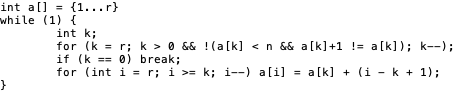
\includegraphics[scale=0.5]{a.png} \end{figure}

\fbox{\textbf{Enum r-subsets of n-set}}
\begin{figure}[h] 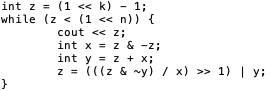
\includegraphics[scale=0.5]{b.png} \end{figure}

\noindent\rule{\linewidth}{1pt}

\fbox{\textbf{Difference table}} leftmost diagonal $= c_0, \hdots c_p, 0, \hdots $ $\rightarrow$ original sequence
\begin{align*}
	h_n &= c_0 \binom{n}{0} + \hdots + c_p \binom{n}{p} \\
	\sum_{k = 0..n}{h_k} &= c_0 \binom{n+1}{1} + \hdots + c_p \binom{n+1}{p+1}
\end{align*}

\noindent\rule{\linewidth}{1pt}

\fbox{\textbf{Catalan number}} \\ $C_n =$ \# $\pm 1$ sequences with non-negative prefix sum
\begin{align*}
	C_n &= \frac{1}{n+1} \binom{2n}{n} \\
	C_n &= \frac{4n-2}{n+1} C_{n-1}
\end{align*}

\noindent\rule{\linewidth}{1pt}

\fbox{\textbf{Stirling-1 number}} \\ $s(p,k) =$ \# $p$ diff items into $k$ same circular permutations
\begin{align*}
	s(p,0) &= 0 & (p \ge 1) \\
	s(p,p) &= 1 & (p \ge 0) \\
	s(p,k) &= (p-1) s(p-1,k) + s(p-1,k-1) & (1 \le k \le p-1) \\
	A_n^p &= \sum_{k = 0..p}{(-1)^{p-k} s(p,k) n^k}
\end{align*}

\fbox{\textbf{Stirling-2 number}} \\ $S(p,k) =$ \# $p$ diff items into $k$ same boxes, no empty box
\begin{align*}
	S(p,0) &= 0 & (p \ge 1) \\
	S(p,p) &= 1 & (p \ge 0) \\
	S(p,k) &= k S(p-1,k) + S(p-1,k-1) & (1 \le k \le p-1) \\
	S(p,k) &= \frac{1}{k!} \sum_{i = 0..k}{(-1)^i \binom{k}{i} (k-i)^p} \\
	n^p &= \sum_{k = 0..p}{S(p,k) A_n^k}
\end{align*}
\# $p$ diff items into $k$ diff boxes $= k! S(p,k)$

\fbox{\textbf{Bell number}} \\ $B_p =$ \# $p$ diff items into same boxes
\begin{align*}
	B_p &= S(p,0) + \hdots + S(p,p) \\
	B_p &= \binom{p-1}{0} B_0 + \hdots + \binom{p-1}{p-1} B_{p-1} \\
	B_{p^i+k} &\equiv i B_k + B_{k+1} \pmod{p}
\end{align*}

\noindent\rule{\linewidth}{1pt}

\fbox{\textbf{Generating function}} \\ % CF258e
$r$-combination: $\prod{(1 + x^1 + x^2 + \hdots + x^{f_i})}$ \\
$r$-arrangement: $r! \prod{(1 + \frac{x^1}{1!} + \frac{x^2}{2!} + \hdots + \frac{x^{f_i}}{f_i!})}$ \\
Integer partition: $\prod_{k = 1..n}{(1-x^k)^{-1}}$

\noindent\rule{\linewidth}{1pt}

\fbox{\textbf{Burnside lemma, Polya enum theorem}} \\
\# inequivalent colorings on $n$-set under a permutation group. 
\begin{equation*}
	N(C,G) = \frac{1}{|G|} \sum_{f \in G}{|C(f)|} = \frac{1}{|G|} \sum_{f \in G}{k^{\#(f)}} = \frac{1}{|G|} \sum_{f \in G}{k^{\sum{e_i}}}
\end{equation*}
$G$ is the equivalent permutation group \\
$C$ is all colorings on $n$-set \\
$N(C,G)$ is \# inequivalent colorings \\
$C(f)$ is the stable kernel of permutation $f$ \\
$k$ is the number of colors available \\
$\#(f)$ is the number of cycles in permutation $f$ \\
$e_1 \hdots e_n$ is the type of permutation $f$ - it has $e_i$ $i$-cycles 

\noindent\rule{\linewidth}{1pt}

\subsection{Graph Theory}

\fbox{\textbf{Havel-Hakimi algo}} \\ degree sequence $(d_1 \ge \hdots \ge d_n)$ is simple-graphic iff $(d_2-1 \hdots d_{d_1+1}-1, d_{d_1+2} \hdots d_n)$ is simple-graphic. Equivalently, connect largest-degree node with other largest-degree nodes. \\
Erdos-Gallai theorem: $(d_1 \ge \hdots \ge d_n)$ is simple-graphic iff
\begin{align*}
	\forall k \in [1,n] \sum_{i=1}^{k}{d_i} \le k(k-1) + \sum_{i=k+1}^{n}{\min{(d_i, k)}}
\end{align*}

\noindent\rule{\linewidth}{1pt}

\fbox{\textbf{Vizing's theorem + Misra-Gries edge coloring algo}} \\ adjacent edges cannot have same color, uses $\max{(deg(v))} + 1$ colors. 

\noindent\rule{\linewidth}{1pt}

\subsection{Game Theory}

\fbox{\textbf{Nim}} Lose iff XOR sum is zero

\noindent\rule{\linewidth}{1pt}

\fbox{\textbf{SG function}} \\
P-position: first lose \\
N-position: second lose \\
Final node must be P \\
N's successors contain at least one P \\
P's successors contain all N \\
$SG(x) = mex(\{SG(y) \mid \text{y is successor of x }\})$ \\
$SG(x) = 0$ iff x is P-position \\
Composite game's SG value is the XOR sum of simple games

\noindent\rule{\linewidth}{1pt}

\subsection{Numerical Methods}

\fbox{\textbf{Newton's method}} solve $f(x) = 0$ by $x \leftarrow x - f(x) / f'(x)$

\noindent\rule{\linewidth}{1pt}

\subsection{Miscellaneous}

\begin{align*}
	\gcd(2^a-1, 2^b-1) &= 2^{\gcd(a,b)}-1
\end{align*}
$x^2 + y^2 = n$ has integer solution $\leftrightarrow$ $n = \prod{p_i^{e_i}}$, there are no $i$ s.t. $p_i \equiv 3 \pmod{4}$ and $e_i \equiv 1 \pmod{2}$

\noindent\rule{\linewidth}{1pt}

\fbox{\textbf{Fibbonacci}}
\begin{align*}
	\gcd(F_n, F_m) &= F_{\gcd(n, m)} \\
	b \mid a &\leftrightarrow F_b \mid F_a
\end{align*}

\noindent\rule{\linewidth}{1pt}

\fbox{\textbf{Derangements}} \\
\begin{align*}
	D_n &= n! (1 - \frac{1}{1!} + \frac{1}{2!} - \hdots + \frac{(-1)^n}{n!}) \\
	D_n &= (n-1)(D_{n-2} + D_{n-1}) \\
	D_n &= n D_{n-1} + (-1)^n
\end{align*}

\fbox{\textbf{Gray sequence}} $G_i = i \text{ xor } (i >> 1)$

\fbox{\textbf{Farey sequence}} sorted $\frac{a}{b}$ $(1 \le a < b \le N, \gcd(a,b) = 1)$
\begin{align*}
	\frac{a_0}{b_0} &= \frac{0}{1} \\
	\frac{a_1}{b_1} &= \frac{1}{N} \\
	\frac{a_n}{b_n} &= \frac{a_{n-1} \lfloor \frac{N+b_{n-2}}{b_{n-1}} \rfloor - a_{n-2}}{b_{n-1} \lfloor \frac{N+b_{n-2}}{b_{n-1}} \rfloor - b_{n-2}}
\end{align*}

\noindent\rule{\linewidth}{1pt}

\fbox{\textbf{Dilworth theorem}} fewest chain split = longest reverse chain

\noindent\rule{\linewidth}{1pt}

\end{multicols}

\end{document}
